\documentclass[aspectratio=169, 10pt]{beamer}
\usetheme{Warsaw}
\usepackage[utf8]{inputenc}
\usepackage[spanish]{babel}
\usepackage{graphicx}
\usepackage{verbatim}
\usepackage{amsmath}
\usepackage{amsfonts}
\usepackage{amssymb}
\usepackage{tgpagella}
\usepackage{hyperref}
%\hypersetup{colorlinks=true, anchorcolor=black, urlcolor = blue, linkcolor=blue, citecolor=blue}
\usefonttheme{serif}

\author{Nelson R. Salinas}
\title{Observatorio diversidad \\ Dise\~no muestral}

%\setbeamercovered{transparent} 
%\setbeamertemplate{navigation symbols}{} 
%\logo{} 
\institute{Jardín Botánico de Bogotá \\ Conservación \textit{in situ}} 
\date{Abril 28, 2025} 
%\subject{Deep learning times series} 
\begin{document}

\begin{frame}
\titlepage
\end{frame}

%#################################################

\begin{frame}{Observatorio de diversidad}

\begin{block}{Objetivo}
Proyectar variables de diversidad a nivel ciudad garantizando un error máximo de estimación.
\end{block}

%\bigskip

\begin{itemize}

\item<2> ¿Cuantas especies de plantas vasculares terrestres por m\textsuperscript{2} existen en Bogotá?

%\bigskip

\item<2> ¿Han ocurrido cambios en diversidad asociados a cambios en el uso del suelo?

\end{itemize}

\end{frame}


%#################################################

\begin{frame}{Observatorio de diversidad}{Diseño de muestreo}
\begin{columns}
\begin{column}{0.5\textwidth}
\begin{itemize}
\item Población estadística: comunidades vegetales terrestres.
\item Variables indicadoras: biomasa y diversidad vegetal por área.
\item Diseño: sistemático post-estratificado.
\end{itemize}
\end{column}
\begin{column}{0.5\textwidth}

\only<1>{
    \begin{center}
    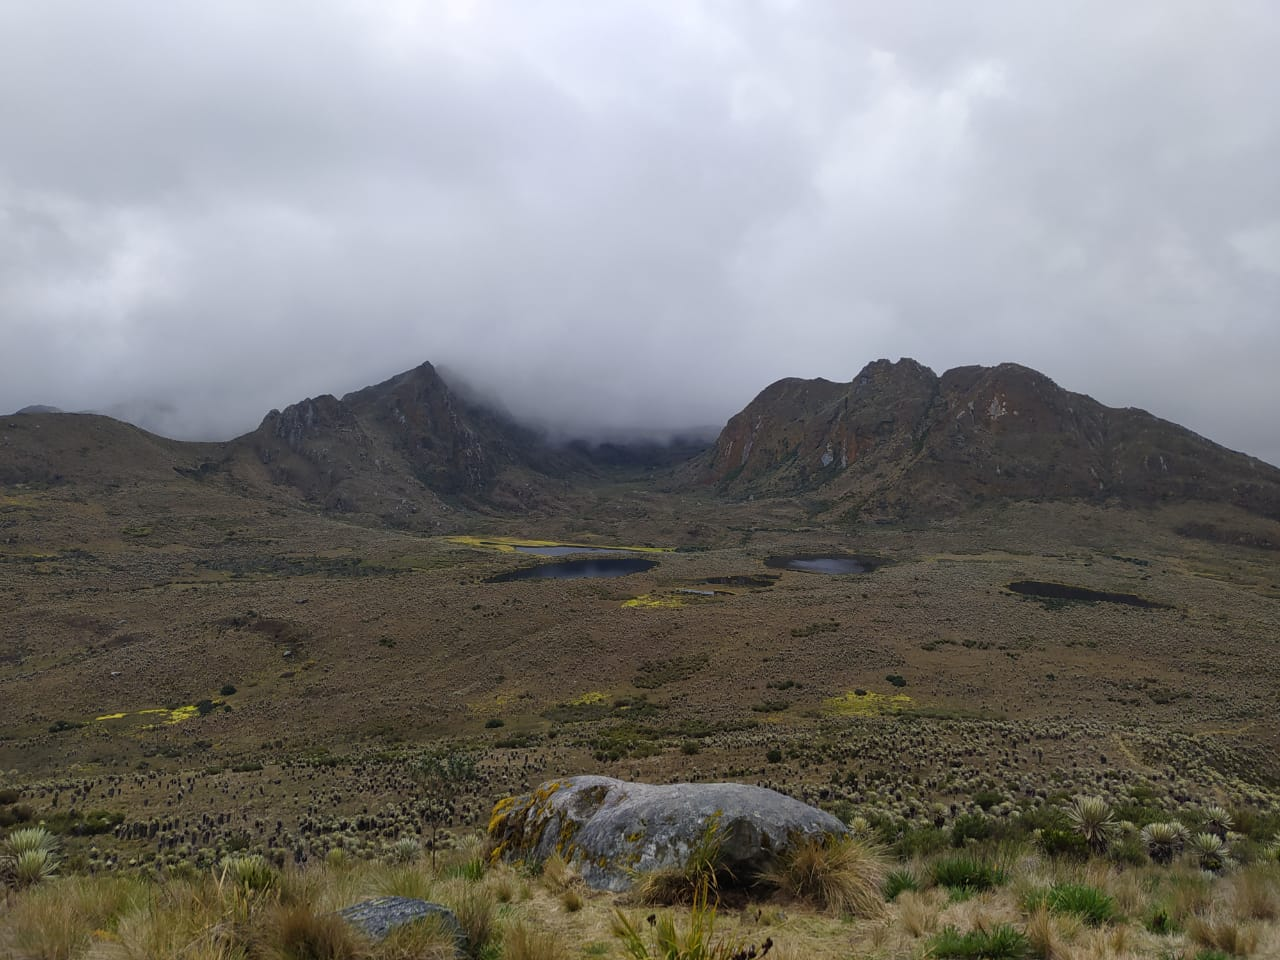
\includegraphics[width=\textwidth]{bocagrande.jpeg} \\
    \hfill { \tiny \textcopyright L. Corrales}
    \end{center}
}

\only<2>{
    \begin{center}
    \includegraphics[width=\textwidth]{mochuelo.jpg} \\
    %\hfill { \tiny \textcopyright L. Corrales}
    \end{center}
}


\end{column}
\end{columns}
\end{frame}
%#################################################
\begin{frame}{Observatorio de diversidad}{Diseño de muestreo}
\begin{columns}
\begin{column}{0.5\textwidth}
\begin{itemize}
\item Marco geoestadistico: cuadrícula 2 $\times$ 2 km.
\item Estratos: coberturas simplificadas CORINE land cover.
\item Probabilidades de selección de muestras: proporcionales a la raíz cuadrada del tamaño del estrato.
\end{itemize}
\end{column}
\begin{column}{0.5\textwidth}

\only<1>{
    \begin{center}
    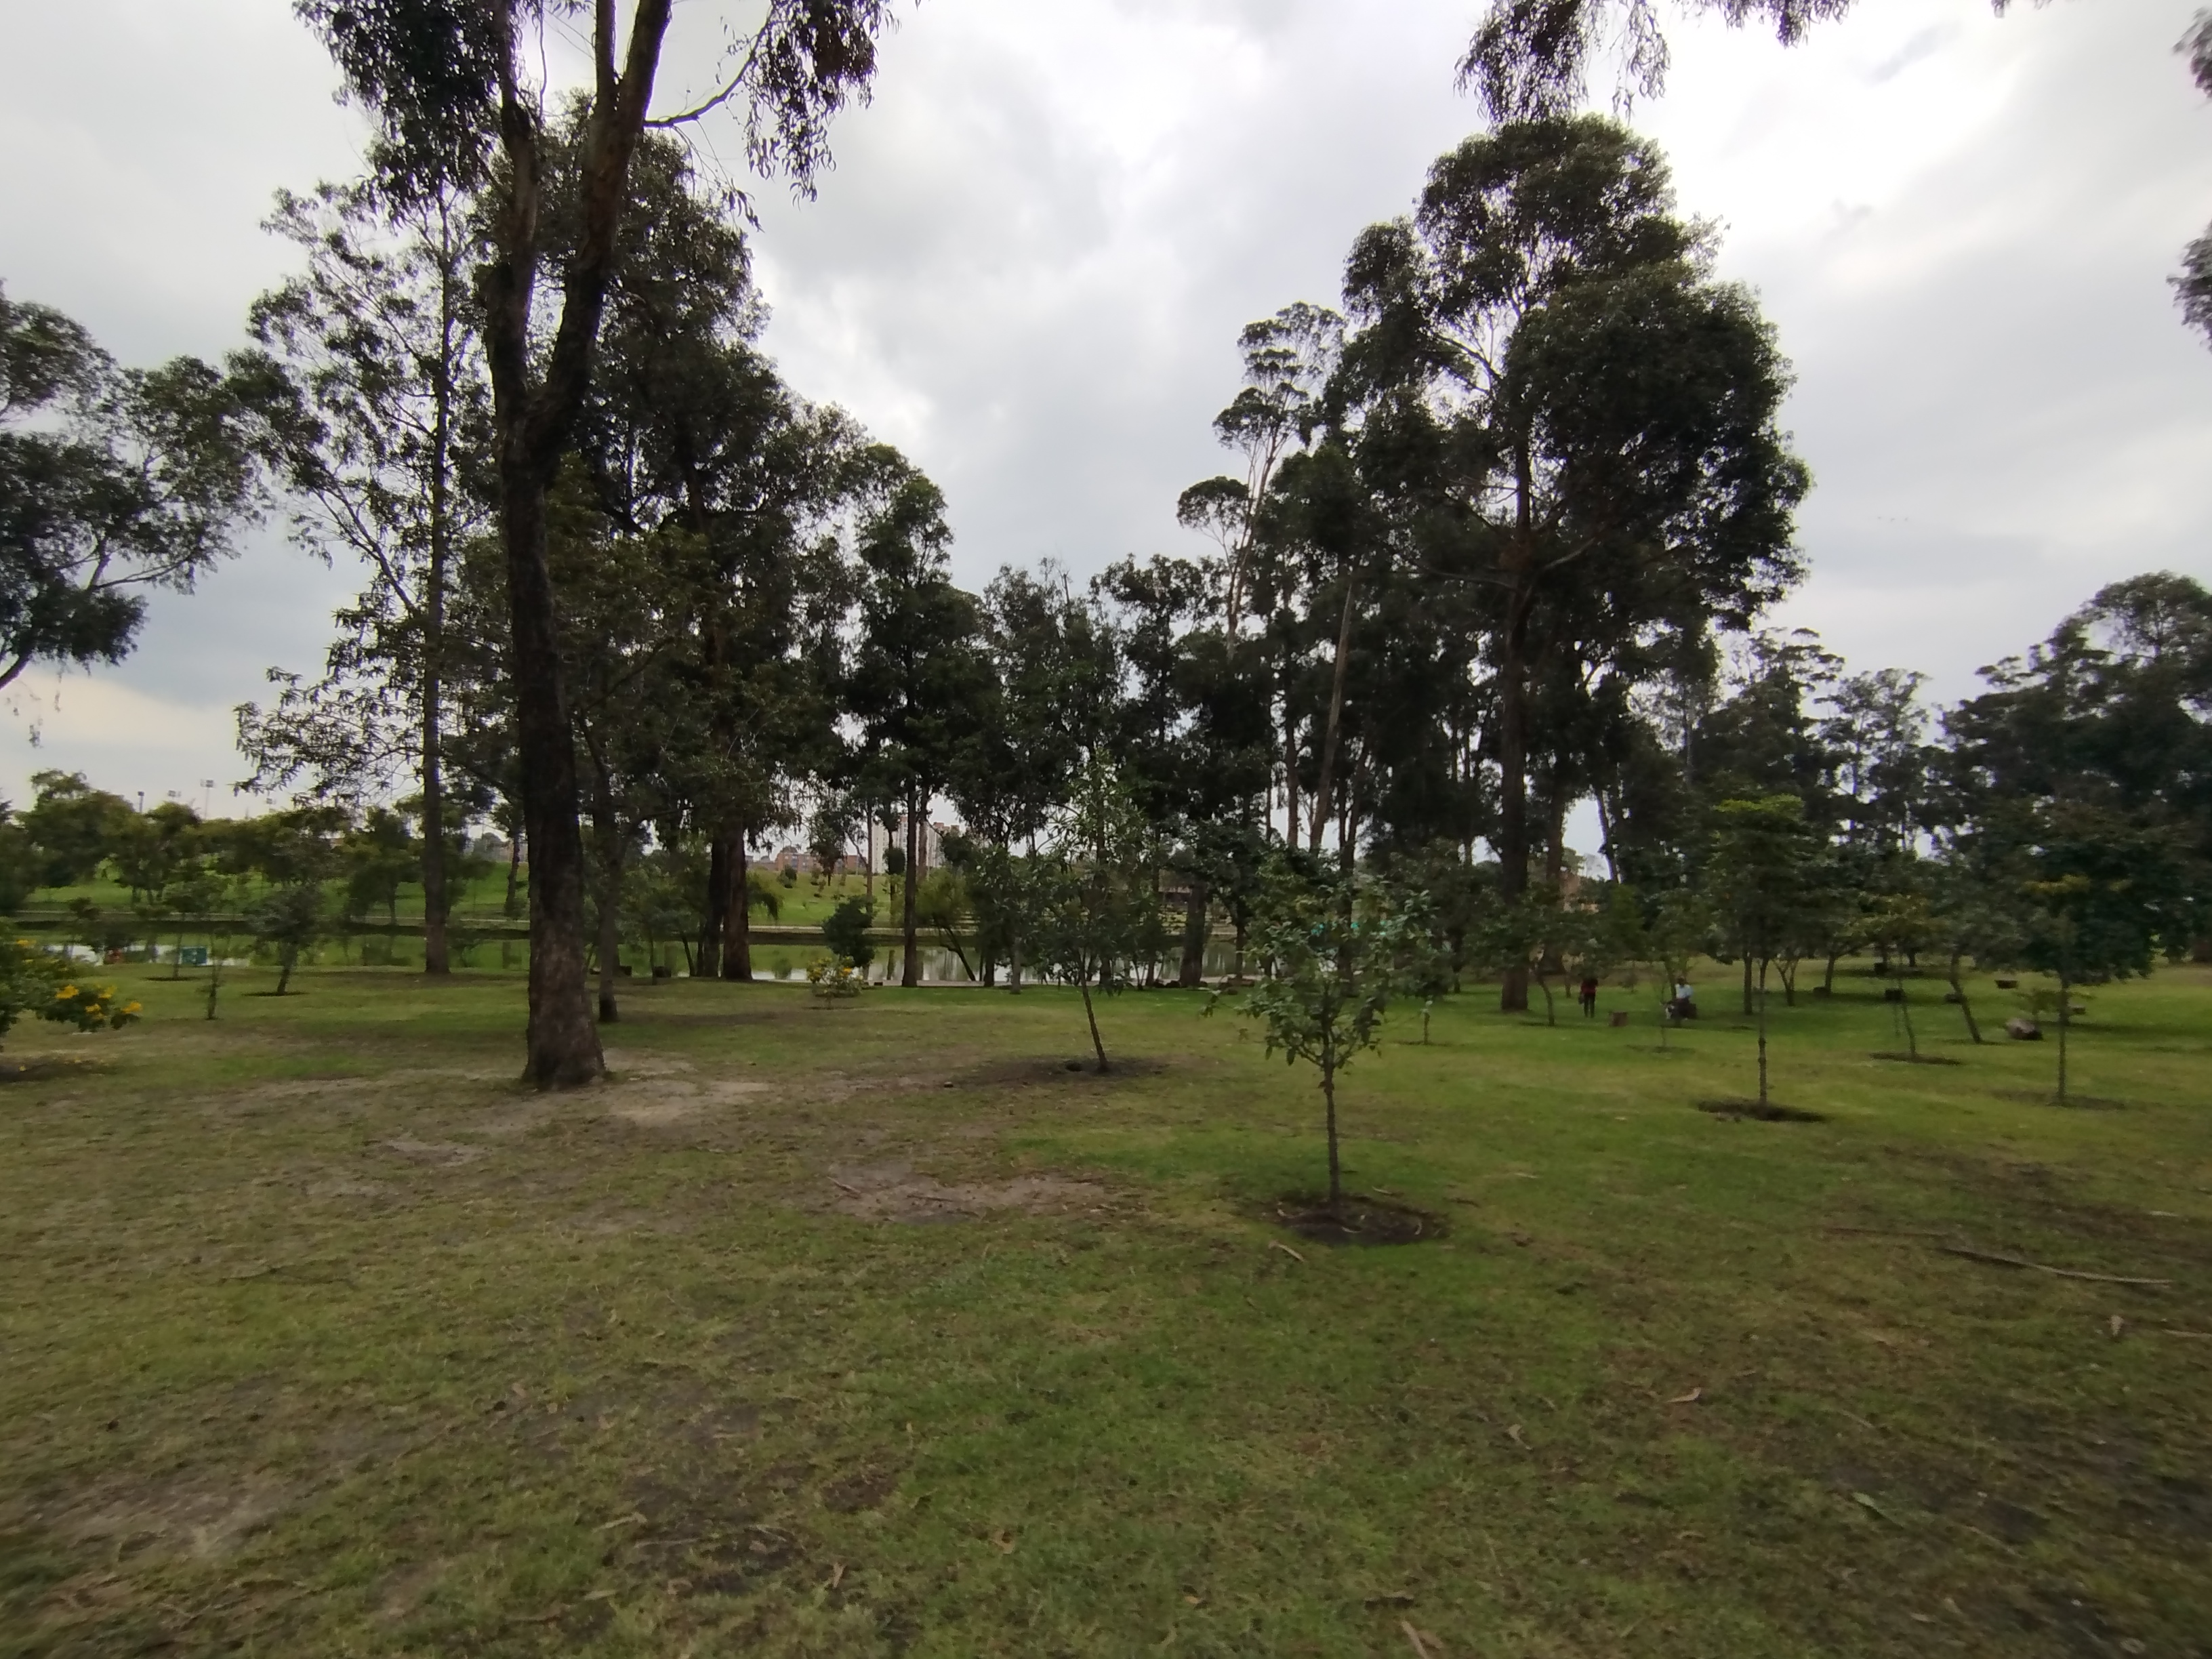
\includegraphics[width=\textwidth]{timiza.jpg} \\
    %\hfill { \tiny \textcopyright L. Corrales}
    \end{center}
}

\only<2>{
    \begin{center}
    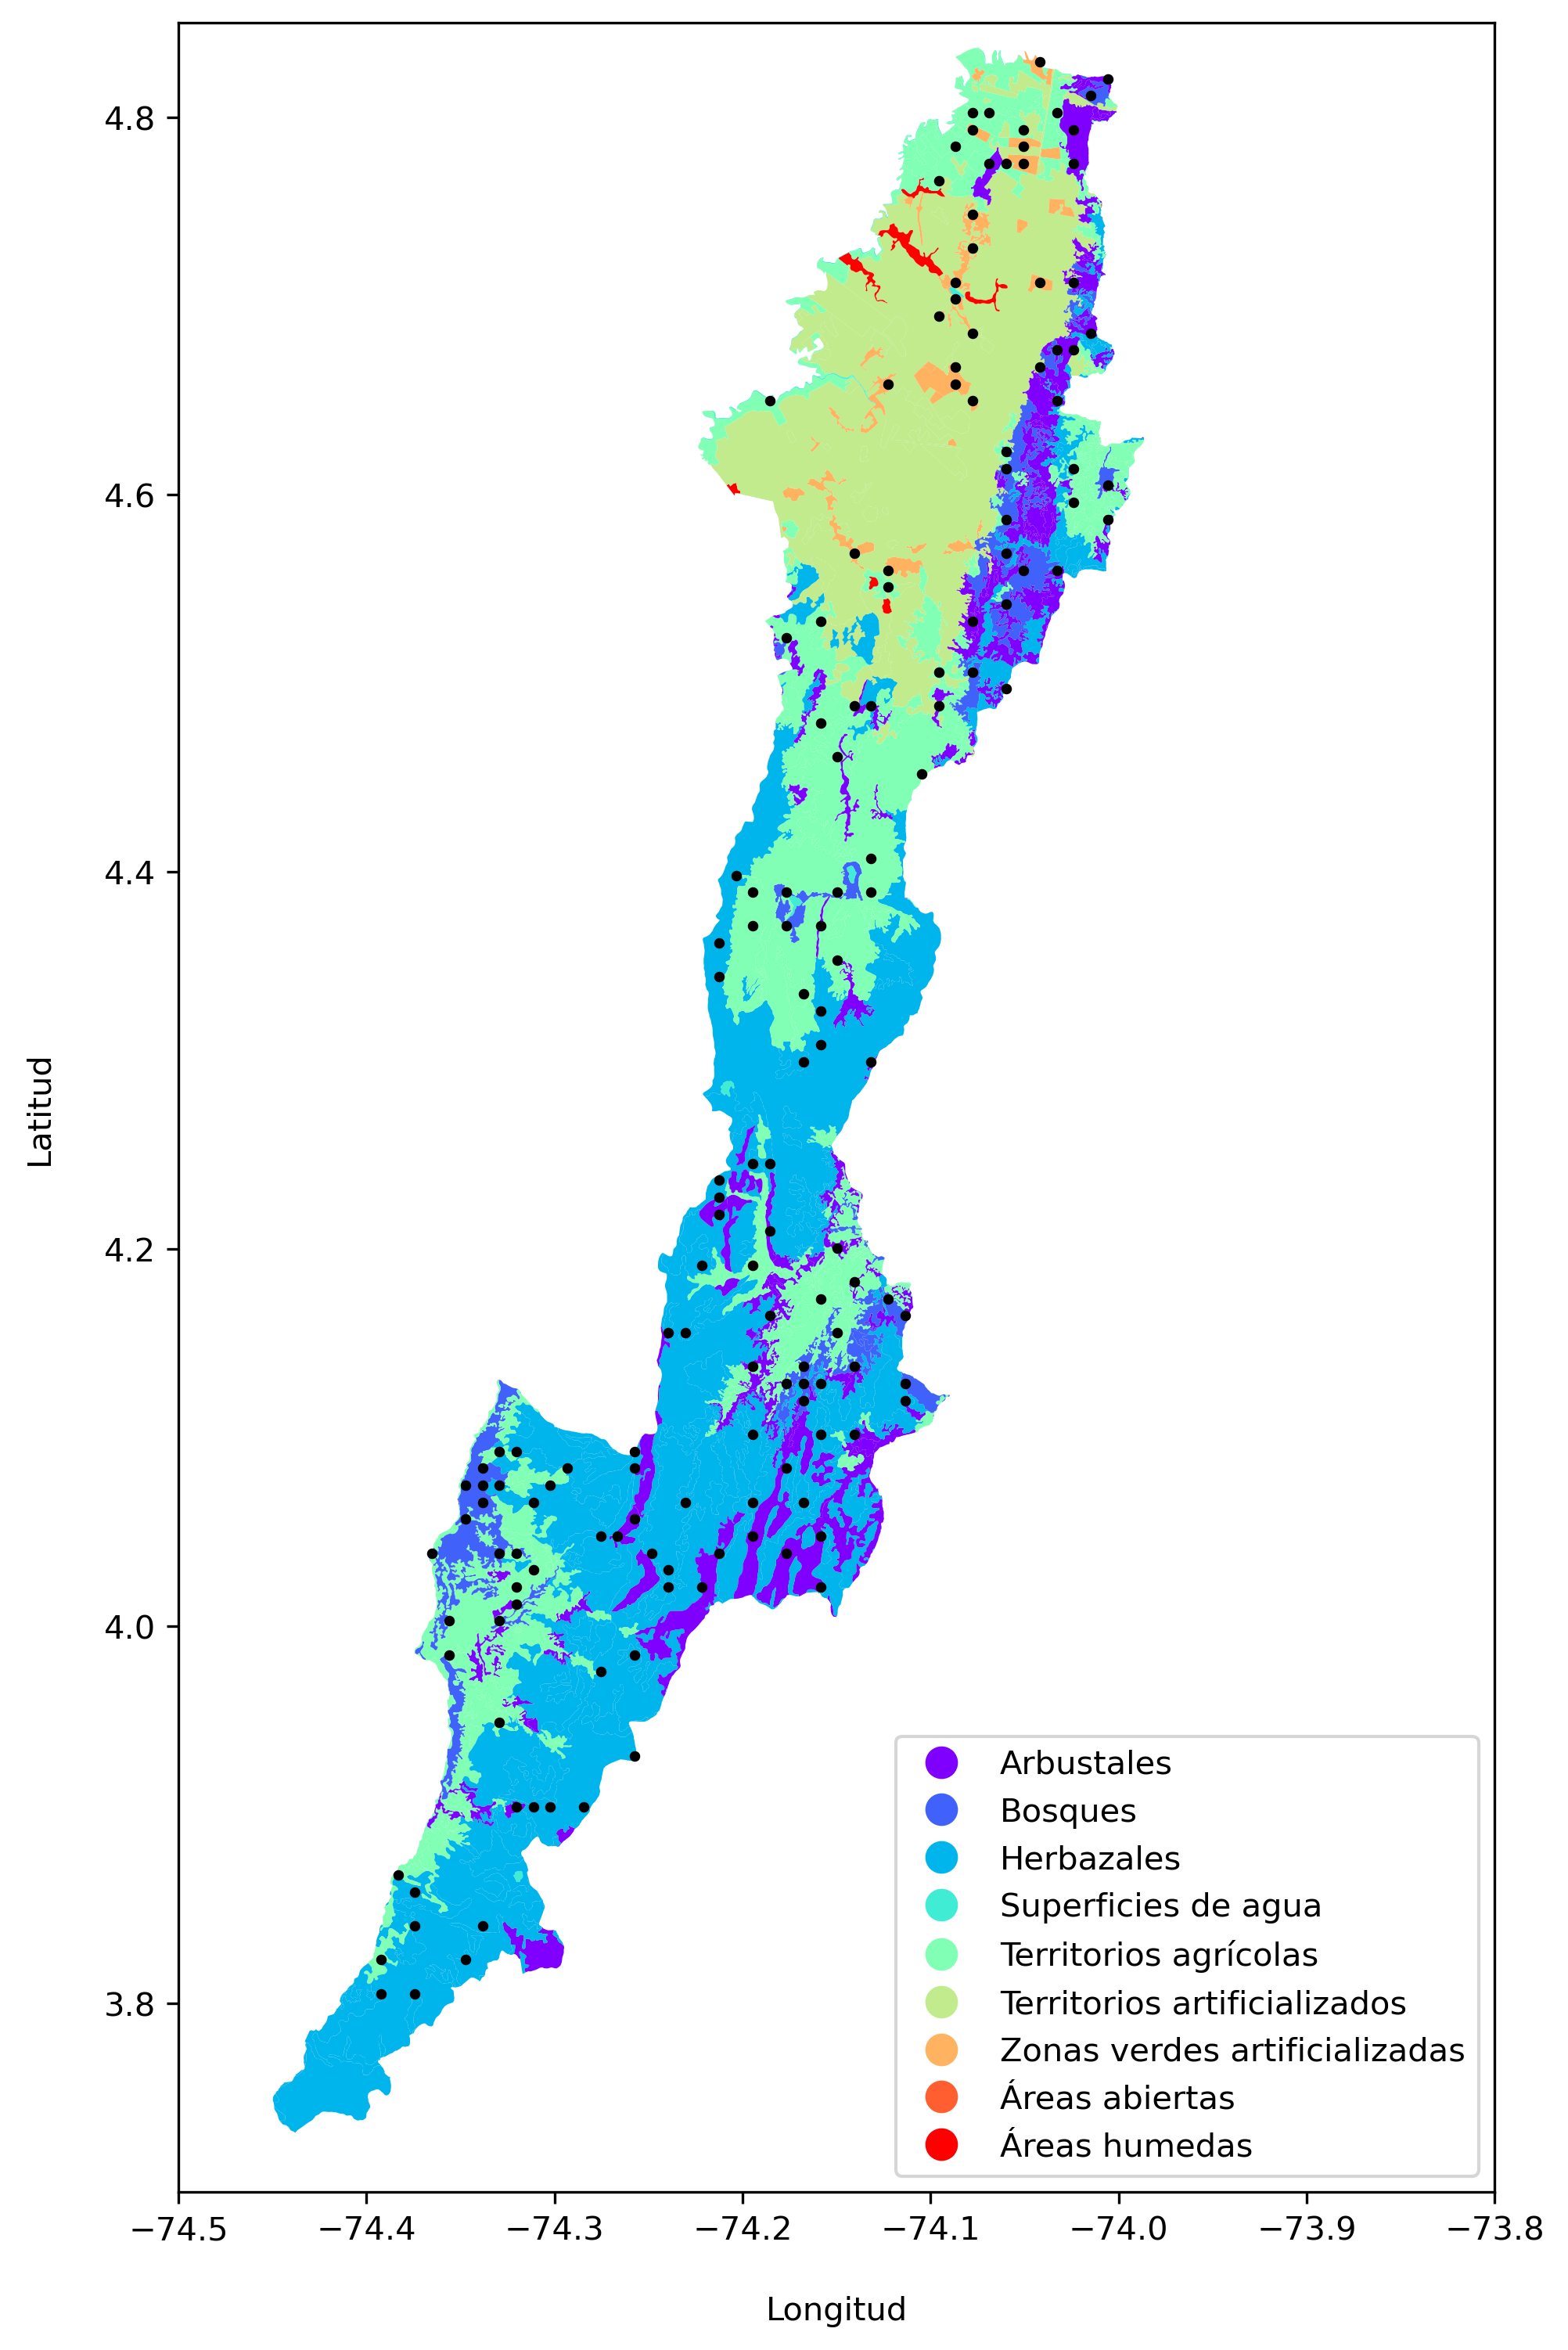
\includegraphics[height=0.8\textheight]{sitios_muestreo.png} \\
    %\hfill { \tiny \textcopyright L. Corrales}
    \end{center}
}

\end{column}
\end{columns}
\end{frame}

%#################################################


\end{document}
